\section{Interfaz 2.00 Menú principal.} \label{inter:interfaz02}
	\subsection{Descripción de la pantalla}
El logotipo del juego se muestra en la parte superior derecha de la pantalla. En la parte inferior izquierda se muestran las dos opciones: Nueva partida, Cargar partida. De fondo se muestra la misma Imagen que en la interfaz 01.00. 
Cada opción desencadena un cuadro de dialogo en donde el usuario debe de confirmar la acción que va desea ejecutar o en donde se le informa que la acción seleccionada no es posible de ejecutar.
	\subsection{Estados del juego}
La interfaz 2.00 contiene los siguientes botones:
\begin{itemize}
	\item \textbf{Nueva partida}:  Dirige a la presentación de la cinemática 1 (ver apartado \ref{Cin:Cinematica01}).
	\item \textbf{Cargar partida}: Dirige a la interfaz 3.00 (ver apartado \ref{inter:interfaz03}) en caso de que exista una partida previamente guardada, en caso contrario abre un cuadro de dialogo en donde se le dice al Jugador que no existe partidas que cargar.
\end{itemize}
Se puede llegar a esta Interfaz a partir de la Interfaz 01.00 (ver apartado \ref{inter:interfaz01})
	\subsection{Imagen}
Ver figura \ref{fig:PMenuP}
\begin{figure}
  \centering
   \subfigure[Menú principal] {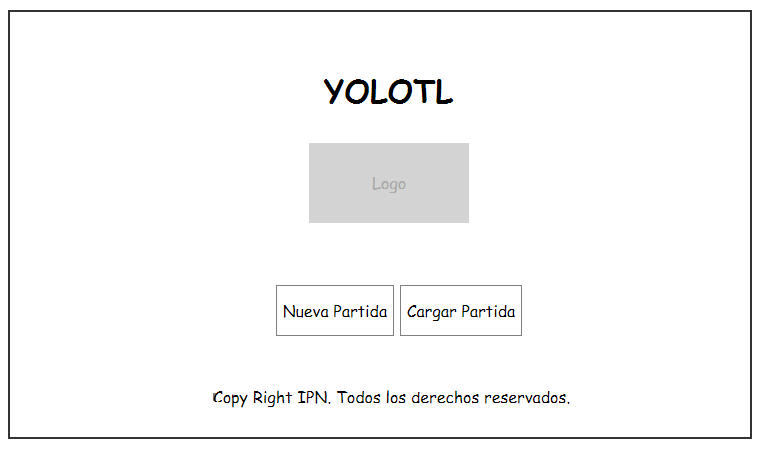
\includegraphics[width=0.6 \textwidth]{Imagenes/interfaz01}}
   
 	\subfigure[Cuadro de dialogo para confirmar iniciar nueva partida.] {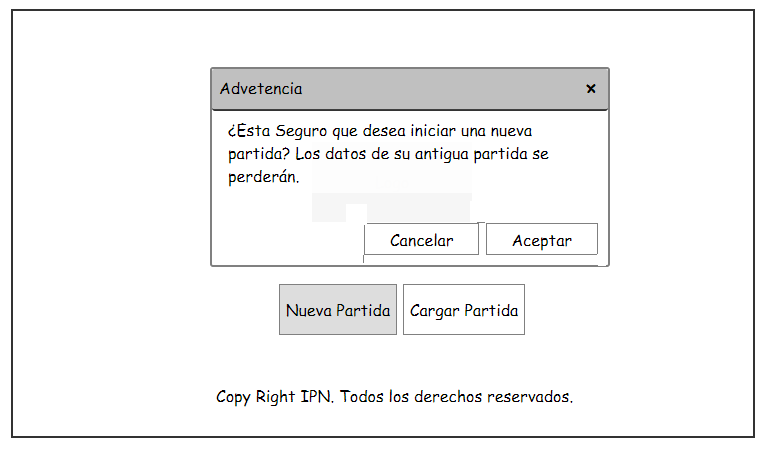
\includegraphics[width=0.6 \textwidth]{Imagenes/interfaz01_02}}
 	
\subfigure[Cuadro de dialogo cuando no existen partidas que cargar.] {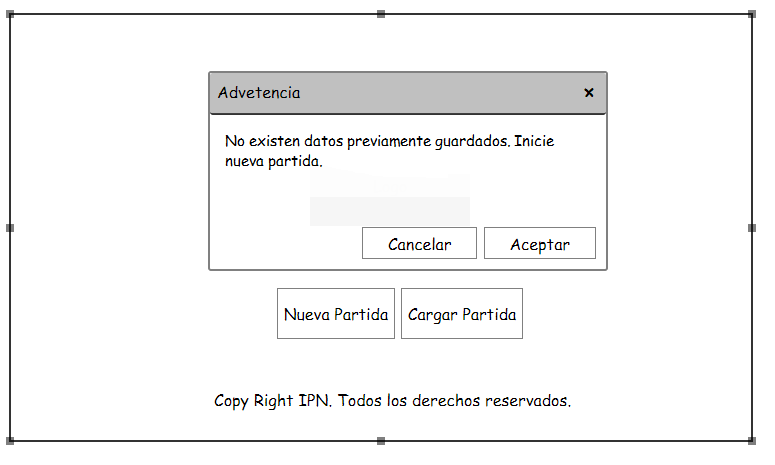
\includegraphics[width=0.6 \textwidth]{Imagenes/interfaz01_03}}
  \caption{Interfaz 2.00 Menú principal.}
  \label{fig:PMenuP}
\end{figure} 